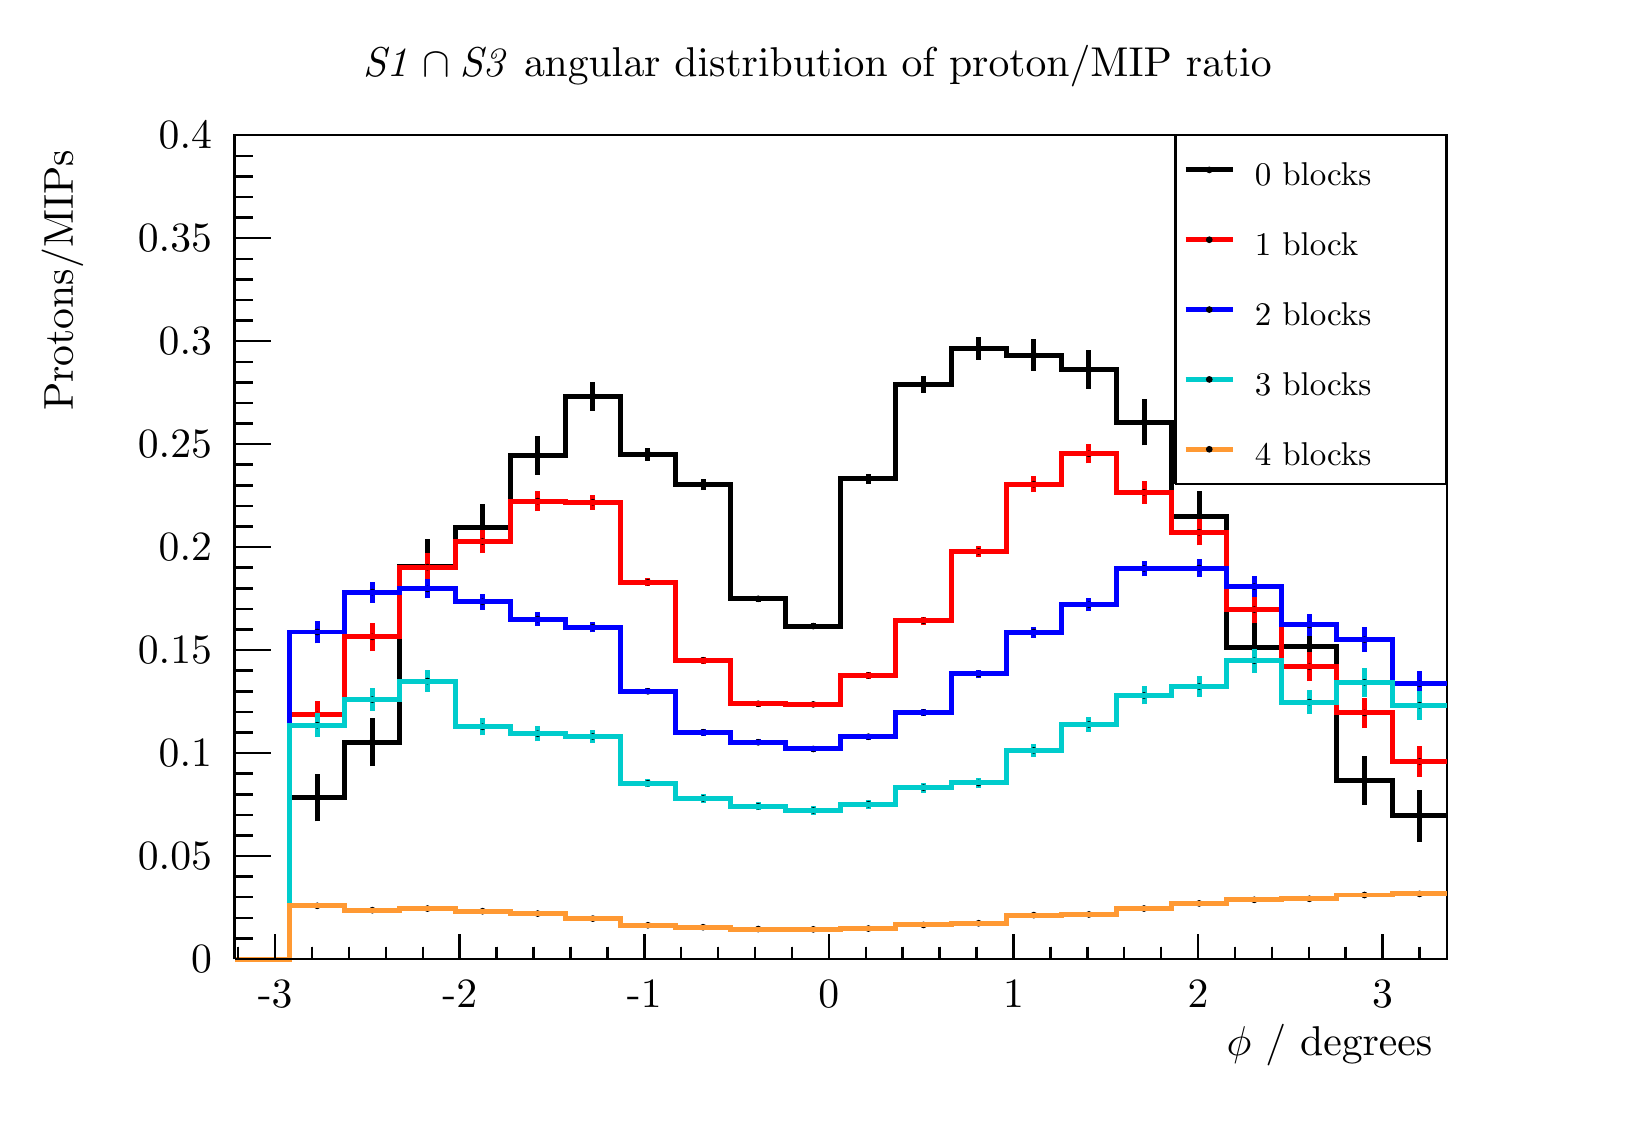
\begin{tikzpicture}
\pgfdeclareplotmark{cross} {
\pgfpathmoveto{\pgfpoint{-0.3\pgfplotmarksize}{\pgfplotmarksize}}
\pgfpathlineto{\pgfpoint{+0.3\pgfplotmarksize}{\pgfplotmarksize}}
\pgfpathlineto{\pgfpoint{+0.3\pgfplotmarksize}{0.3\pgfplotmarksize}}
\pgfpathlineto{\pgfpoint{+1\pgfplotmarksize}{0.3\pgfplotmarksize}}
\pgfpathlineto{\pgfpoint{+1\pgfplotmarksize}{-0.3\pgfplotmarksize}}
\pgfpathlineto{\pgfpoint{+0.3\pgfplotmarksize}{-0.3\pgfplotmarksize}}
\pgfpathlineto{\pgfpoint{+0.3\pgfplotmarksize}{-1.\pgfplotmarksize}}
\pgfpathlineto{\pgfpoint{-0.3\pgfplotmarksize}{-1.\pgfplotmarksize}}
\pgfpathlineto{\pgfpoint{-0.3\pgfplotmarksize}{-0.3\pgfplotmarksize}}
\pgfpathlineto{\pgfpoint{-1.\pgfplotmarksize}{-0.3\pgfplotmarksize}}
\pgfpathlineto{\pgfpoint{-1.\pgfplotmarksize}{0.3\pgfplotmarksize}}
\pgfpathlineto{\pgfpoint{-0.3\pgfplotmarksize}{0.3\pgfplotmarksize}}
\pgfpathclose
\pgfusepathqstroke
}
\pgfdeclareplotmark{cross*} {
\pgfpathmoveto{\pgfpoint{-0.3\pgfplotmarksize}{\pgfplotmarksize}}
\pgfpathlineto{\pgfpoint{+0.3\pgfplotmarksize}{\pgfplotmarksize}}
\pgfpathlineto{\pgfpoint{+0.3\pgfplotmarksize}{0.3\pgfplotmarksize}}
\pgfpathlineto{\pgfpoint{+1\pgfplotmarksize}{0.3\pgfplotmarksize}}
\pgfpathlineto{\pgfpoint{+1\pgfplotmarksize}{-0.3\pgfplotmarksize}}
\pgfpathlineto{\pgfpoint{+0.3\pgfplotmarksize}{-0.3\pgfplotmarksize}}
\pgfpathlineto{\pgfpoint{+0.3\pgfplotmarksize}{-1.\pgfplotmarksize}}
\pgfpathlineto{\pgfpoint{-0.3\pgfplotmarksize}{-1.\pgfplotmarksize}}
\pgfpathlineto{\pgfpoint{-0.3\pgfplotmarksize}{-0.3\pgfplotmarksize}}
\pgfpathlineto{\pgfpoint{-1.\pgfplotmarksize}{-0.3\pgfplotmarksize}}
\pgfpathlineto{\pgfpoint{-1.\pgfplotmarksize}{0.3\pgfplotmarksize}}
\pgfpathlineto{\pgfpoint{-0.3\pgfplotmarksize}{0.3\pgfplotmarksize}}
\pgfpathclose
\pgfusepathqfillstroke
}
\pgfdeclareplotmark{newstar} {
\pgfpathmoveto{\pgfqpoint{0pt}{\pgfplotmarksize}}
\pgfpathlineto{\pgfqpointpolar{44}{0.5\pgfplotmarksize}}
\pgfpathlineto{\pgfqpointpolar{18}{\pgfplotmarksize}}
\pgfpathlineto{\pgfqpointpolar{-20}{0.5\pgfplotmarksize}}
\pgfpathlineto{\pgfqpointpolar{-54}{\pgfplotmarksize}}
\pgfpathlineto{\pgfqpointpolar{-90}{0.5\pgfplotmarksize}}
\pgfpathlineto{\pgfqpointpolar{234}{\pgfplotmarksize}}
\pgfpathlineto{\pgfqpointpolar{198}{0.5\pgfplotmarksize}}
\pgfpathlineto{\pgfqpointpolar{162}{\pgfplotmarksize}}
\pgfpathlineto{\pgfqpointpolar{134}{0.5\pgfplotmarksize}}
\pgfpathclose
\pgfusepathqstroke
}
\pgfdeclareplotmark{newstar*} {
\pgfpathmoveto{\pgfqpoint{0pt}{\pgfplotmarksize}}
\pgfpathlineto{\pgfqpointpolar{44}{0.5\pgfplotmarksize}}
\pgfpathlineto{\pgfqpointpolar{18}{\pgfplotmarksize}}
\pgfpathlineto{\pgfqpointpolar{-20}{0.5\pgfplotmarksize}}
\pgfpathlineto{\pgfqpointpolar{-54}{\pgfplotmarksize}}
\pgfpathlineto{\pgfqpointpolar{-90}{0.5\pgfplotmarksize}}
\pgfpathlineto{\pgfqpointpolar{234}{\pgfplotmarksize}}
\pgfpathlineto{\pgfqpointpolar{198}{0.5\pgfplotmarksize}}
\pgfpathlineto{\pgfqpointpolar{162}{\pgfplotmarksize}}
\pgfpathlineto{\pgfqpointpolar{134}{0.5\pgfplotmarksize}}
\pgfpathclose
\pgfusepathqfillstroke
}
\definecolor{c}{rgb}{1,1,1};
\draw [color=c, fill=c] (0,0) rectangle (20,13.5876);
\draw [color=c, fill=c] (2.6,1.76638) rectangle (18,12.2288);
\definecolor{c}{rgb}{0,0,0};
\draw [c,line width=0.9] (2.6,1.76638) -- (2.6,12.2288) -- (18,12.2288) -- (18,1.76638) -- (2.6,1.76638);
\definecolor{c}{rgb}{1,1,1};
\draw [color=c, fill=c] (2.6,1.76638) rectangle (18,12.2288);
\definecolor{c}{rgb}{0,0,0};
\draw [c,line width=0.9] (2.6,1.76638) -- (2.6,12.2288) -- (18,12.2288) -- (18,1.76638) -- (2.6,1.76638);
\definecolor{c}{rgb}{0,0,0.6};
\draw [c,line width=0.9] (2.6,1.76638) -- (3.3,1.76638) -- (3.3,1.76638) -- (4,1.76638) -- (4,1.76638) -- (4.7,1.76638) -- (4.7,1.76638) -- (5.4,1.76638) -- (5.4,1.76638) -- (6.1,1.76638) -- (6.1,1.76638) -- (6.8,1.76638) -- (6.8,1.76638) --
 (7.5,1.76638) -- (7.5,1.76638) -- (8.2,1.76638) -- (8.2,1.76638) -- (8.9,1.76638) -- (8.9,1.76638) -- (9.6,1.76638) -- (9.6,1.76638) -- (10.3,1.76638) -- (10.3,1.76638) -- (11,1.76638) -- (11,1.76638) -- (11.7,1.76638) -- (11.7,1.76638) --
 (12.4,1.76638) -- (12.4,1.76638) -- (13.1,1.76638) -- (13.1,1.76638) -- (13.8,1.76638) -- (13.8,1.76638) -- (14.5,1.76638) -- (14.5,1.76638) -- (15.2,1.76638) -- (15.2,1.76638) -- (15.9,1.76638) -- (15.9,1.76638) -- (16.6,1.76638) -- (16.6,1.76638)
 -- (17.3,1.76638) -- (17.3,1.76638) -- (18,1.76638);
\definecolor{c}{rgb}{0,0,0};
\draw [c,line width=0.9] (2.6,1.76638) -- (18,1.76638);
\draw [c,line width=0.9] (3.11568,2.08026) -- (3.11568,1.76638);
\draw [c,line width=0.9] (3.58447,1.92332) -- (3.58447,1.76638);
\draw [c,line width=0.9] (4.05327,1.92332) -- (4.05327,1.76638);
\draw [c,line width=0.9] (4.52207,1.92332) -- (4.52207,1.76638);
\draw [c,line width=0.9] (4.99087,1.92332) -- (4.99087,1.76638);
\draw [c,line width=0.9] (5.45967,2.08026) -- (5.45967,1.76638);
\draw [c,line width=0.9] (5.92846,1.92332) -- (5.92846,1.76638);
\draw [c,line width=0.9] (6.39726,1.92332) -- (6.39726,1.76638);
\draw [c,line width=0.9] (6.86606,1.92332) -- (6.86606,1.76638);
\draw [c,line width=0.9] (7.33486,1.92332) -- (7.33486,1.76638);
\draw [c,line width=0.9] (7.80365,2.08026) -- (7.80365,1.76638);
\draw [c,line width=0.9] (8.27245,1.92332) -- (8.27245,1.76638);
\draw [c,line width=0.9] (8.74125,1.92332) -- (8.74125,1.76638);
\draw [c,line width=0.9] (9.21005,1.92332) -- (9.21005,1.76638);
\draw [c,line width=0.9] (9.67884,1.92332) -- (9.67884,1.76638);
\draw [c,line width=0.9] (10.1476,2.08026) -- (10.1476,1.76638);
\draw [c,line width=0.9] (10.6164,1.92332) -- (10.6164,1.76638);
\draw [c,line width=0.9] (11.0852,1.92332) -- (11.0852,1.76638);
\draw [c,line width=0.9] (11.554,1.92332) -- (11.554,1.76638);
\draw [c,line width=0.9] (12.0228,1.92332) -- (12.0228,1.76638);
\draw [c,line width=0.9] (12.4916,2.08026) -- (12.4916,1.76638);
\draw [c,line width=0.9] (12.9604,1.92332) -- (12.9604,1.76638);
\draw [c,line width=0.9] (13.4292,1.92332) -- (13.4292,1.76638);
\draw [c,line width=0.9] (13.898,1.92332) -- (13.898,1.76638);
\draw [c,line width=0.9] (14.3668,1.92332) -- (14.3668,1.76638);
\draw [c,line width=0.9] (14.8356,2.08026) -- (14.8356,1.76638);
\draw [c,line width=0.9] (15.3044,1.92332) -- (15.3044,1.76638);
\draw [c,line width=0.9] (15.7732,1.92332) -- (15.7732,1.76638);
\draw [c,line width=0.9] (16.242,1.92332) -- (16.242,1.76638);
\draw [c,line width=0.9] (16.7108,1.92332) -- (16.7108,1.76638);
\draw [c,line width=0.9] (17.1796,2.08026) -- (17.1796,1.76638);
\draw [c,line width=0.9] (3.11568,2.08026) -- (3.11568,1.76638);
\draw [c,line width=0.9] (2.64688,1.92332) -- (2.64688,1.76638);
\draw [c,line width=0.9] (17.1796,2.08026) -- (17.1796,1.76638);
\draw [c,line width=0.9] (17.6484,1.92332) -- (17.6484,1.76638);
\draw [anchor=base] (3.11568,1.15494) node[scale=1.50574, color=c, rotate=0]{-3};
\draw [anchor=base] (5.45967,1.15494) node[scale=1.50574, color=c, rotate=0]{-2};
\draw [anchor=base] (7.80365,1.15494) node[scale=1.50574, color=c, rotate=0]{-1};
\draw [anchor=base] (10.1476,1.15494) node[scale=1.50574, color=c, rotate=0]{0};
\draw [anchor=base] (12.4916,1.15494) node[scale=1.50574, color=c, rotate=0]{1};
\draw [anchor=base] (14.8356,1.15494) node[scale=1.50574, color=c, rotate=0]{2};
\draw [anchor=base] (17.1796,1.15494) node[scale=1.50574, color=c, rotate=0]{3};
\draw [anchor= east] (18,0.679378) node[scale=1.50574, color=c, rotate=0]{$\phi$ / degrees};
\draw [c,line width=0.9] (2.6,1.76638) -- (2.6,12.2288);
\draw [c,line width=0.9] (3.062,1.76638) -- (2.6,1.76638);
\draw [c,line width=0.9] (2.831,2.02794) -- (2.6,2.02794);
\draw [c,line width=0.9] (2.831,2.28951) -- (2.6,2.28951);
\draw [c,line width=0.9] (2.831,2.55107) -- (2.6,2.55107);
\draw [c,line width=0.9] (2.831,2.81263) -- (2.6,2.81263);
\draw [c,line width=0.9] (3.062,3.07419) -- (2.6,3.07419);
\draw [c,line width=0.9] (2.831,3.33575) -- (2.6,3.33575);
\draw [c,line width=0.9] (2.831,3.59731) -- (2.6,3.59731);
\draw [c,line width=0.9] (2.831,3.85887) -- (2.6,3.85887);
\draw [c,line width=0.9] (2.831,4.12043) -- (2.6,4.12043);
\draw [c,line width=0.9] (3.062,4.38199) -- (2.6,4.38199);
\draw [c,line width=0.9] (2.831,4.64355) -- (2.6,4.64355);
\draw [c,line width=0.9] (2.831,4.90511) -- (2.6,4.90511);
\draw [c,line width=0.9] (2.831,5.16667) -- (2.6,5.16667);
\draw [c,line width=0.9] (2.831,5.42823) -- (2.6,5.42823);
\draw [c,line width=0.9] (3.062,5.6898) -- (2.6,5.6898);
\draw [c,line width=0.9] (2.831,5.95136) -- (2.6,5.95136);
\draw [c,line width=0.9] (2.831,6.21292) -- (2.6,6.21292);
\draw [c,line width=0.9] (2.831,6.47448) -- (2.6,6.47448);
\draw [c,line width=0.9] (2.831,6.73604) -- (2.6,6.73604);
\draw [c,line width=0.9] (3.062,6.9976) -- (2.6,6.9976);
\draw [c,line width=0.9] (2.831,7.25916) -- (2.6,7.25916);
\draw [c,line width=0.9] (2.831,7.52072) -- (2.6,7.52072);
\draw [c,line width=0.9] (2.831,7.78228) -- (2.6,7.78228);
\draw [c,line width=0.9] (2.831,8.04384) -- (2.6,8.04384);
\draw [c,line width=0.9] (3.062,8.3054) -- (2.6,8.3054);
\draw [c,line width=0.9] (2.831,8.56696) -- (2.6,8.56696);
\draw [c,line width=0.9] (2.831,8.82852) -- (2.6,8.82852);
\draw [c,line width=0.9] (2.831,9.09008) -- (2.6,9.09008);
\draw [c,line width=0.9] (2.831,9.35165) -- (2.6,9.35165);
\draw [c,line width=0.9] (3.062,9.61321) -- (2.6,9.61321);
\draw [c,line width=0.9] (2.831,9.87477) -- (2.6,9.87477);
\draw [c,line width=0.9] (2.831,10.1363) -- (2.6,10.1363);
\draw [c,line width=0.9] (2.831,10.3979) -- (2.6,10.3979);
\draw [c,line width=0.9] (2.831,10.6594) -- (2.6,10.6594);
\draw [c,line width=0.9] (3.062,10.921) -- (2.6,10.921);
\draw [c,line width=0.9] (2.831,11.1826) -- (2.6,11.1826);
\draw [c,line width=0.9] (2.831,11.4441) -- (2.6,11.4441);
\draw [c,line width=0.9] (2.831,11.7057) -- (2.6,11.7057);
\draw [c,line width=0.9] (2.831,11.9673) -- (2.6,11.9673);
\draw [c,line width=0.9] (3.062,12.2288) -- (2.6,12.2288);
\draw [anchor= east] (2.5,1.76638) node[scale=1.50574, color=c, rotate=0]{0};
\draw [anchor= east] (2.5,3.07419) node[scale=1.50574, color=c, rotate=0]{0.05};
\draw [anchor= east] (2.5,4.38199) node[scale=1.50574, color=c, rotate=0]{0.1};
\draw [anchor= east] (2.5,5.6898) node[scale=1.50574, color=c, rotate=0]{0.15};
\draw [anchor= east] (2.5,6.9976) node[scale=1.50574, color=c, rotate=0]{0.2};
\draw [anchor= east] (2.5,8.3054) node[scale=1.50574, color=c, rotate=0]{0.25};
\draw [anchor= east] (2.5,9.61321) node[scale=1.50574, color=c, rotate=0]{0.3};
\draw [anchor= east] (2.5,10.921) node[scale=1.50574, color=c, rotate=0]{0.35};
\draw [anchor= east] (2.5,12.2288) node[scale=1.50574, color=c, rotate=0]{0.4};
\draw [anchor= east] (0.413559,12.2288) node[scale=1.50574, color=c, rotate=90]{  Protons/MIPs};
\draw [c,line width=1.8] (3.65,3.51506) -- (3.65,3.81731);
\draw [c,line width=1.8] (3.65,3.81731) -- (3.65,4.11956);
\foreach \P in {(3.65,3.81731)}{\draw[mark options={color=c,fill=c},mark size=2.402402pt,mark=*,mark size=1pt] plot coordinates {\P};}
\draw [c,line width=1.8] (4.35,4.21512) -- (4.35,4.52157);
\draw [c,line width=1.8] (4.35,4.52157) -- (4.35,4.82801);
\foreach \P in {(4.35,4.52157)}{\draw[mark options={color=c,fill=c},mark size=2.402402pt,mark=*,mark size=1pt] plot coordinates {\P};}
\draw [c,line width=1.8] (5.05,6.41471) -- (5.05,6.75637);
\draw [c,line width=1.8] (5.05,6.75637) -- (5.05,7.09804);
\foreach \P in {(5.05,6.75637)}{\draw[mark options={color=c,fill=c},mark size=2.402402pt,mark=*,mark size=1pt] plot coordinates {\P};}
\draw [c,line width=1.8] (5.75,6.95517) -- (5.75,7.25022);
\draw [c,line width=1.8] (5.75,7.25022) -- (5.75,7.54527);
\foreach \P in {(5.75,7.25022)}{\draw[mark options={color=c,fill=c},mark size=2.402402pt,mark=*,mark size=1pt] plot coordinates {\P};}
\draw [c,line width=1.8] (6.45,7.91644) -- (6.45,8.16457);
\draw [c,line width=1.8] (6.45,8.16457) -- (6.45,8.4127);
\foreach \P in {(6.45,8.16457)}{\draw[mark options={color=c,fill=c},mark size=2.402402pt,mark=*,mark size=1pt] plot coordinates {\P};}
\draw [c,line width=1.8] (7.15,8.73239) -- (7.15,8.91519);
\draw [c,line width=1.8] (7.15,8.91519) -- (7.15,9.09799);
\foreach \P in {(7.15,8.91519)}{\draw[mark options={color=c,fill=c},mark size=2.402402pt,mark=*,mark size=1pt] plot coordinates {\P};}
\draw [c,line width=1.8] (7.85,8.0915) -- (7.85,8.17703);
\draw [c,line width=1.8] (7.85,8.17703) -- (7.85,8.26256);
\foreach \P in {(7.85,8.17703)}{\draw[mark options={color=c,fill=c},mark size=2.402402pt,mark=*,mark size=1pt] plot coordinates {\P};}
\draw [c,line width=1.8] (8.55,7.72165) -- (8.55,7.79397);
\draw [c,line width=1.8] (8.55,7.79397) -- (8.55,7.86628);
\foreach \P in {(8.55,7.79397)}{\draw[mark options={color=c,fill=c},mark size=2.402402pt,mark=*,mark size=1pt] plot coordinates {\P};}
\draw [c,line width=1.8] (9.25,6.30183) -- (9.25,6.34125);
\draw [c,line width=1.8] (9.25,6.34125) -- (9.25,6.38067);
\foreach \P in {(9.25,6.34125)}{\draw[mark options={color=c,fill=c},mark size=2.402402pt,mark=*,mark size=1pt] plot coordinates {\P};}
\draw [c,line width=1.8] (9.95,5.95924) -- (9.95,5.99463);
\draw [c,line width=1.8] (9.95,5.99463) -- (9.95,6.03002);
\foreach \P in {(9.95,5.99463)}{\draw[mark options={color=c,fill=c},mark size=2.402402pt,mark=*,mark size=1pt] plot coordinates {\P};}
\draw [c,line width=1.8] (10.65,7.80545) -- (10.65,7.86821);
\draw [c,line width=1.8] (10.65,7.86821) -- (10.65,7.93096);
\foreach \P in {(10.65,7.86821)}{\draw[mark options={color=c,fill=c},mark size=2.402402pt,mark=*,mark size=1pt] plot coordinates {\P};}
\draw [c,line width=1.8] (11.35,8.95798) -- (11.35,9.06275);
\draw [c,line width=1.8] (11.35,9.06275) -- (11.35,9.16752);
\foreach \P in {(11.35,9.06275)}{\draw[mark options={color=c,fill=c},mark size=2.402402pt,mark=*,mark size=1pt] plot coordinates {\P};}
\draw [c,line width=1.8] (12.05,9.37401) -- (12.05,9.52022);
\draw [c,line width=1.8] (12.05,9.52022) -- (12.05,9.66644);
\foreach \P in {(12.05,9.52022)}{\draw[mark options={color=c,fill=c},mark size=2.402402pt,mark=*,mark size=1pt] plot coordinates {\P};}
\draw [c,line width=1.8] (12.75,9.23657) -- (12.75,9.43564);
\draw [c,line width=1.8] (12.75,9.43564) -- (12.75,9.63472);
\foreach \P in {(12.75,9.43564)}{\draw[mark options={color=c,fill=c},mark size=2.402402pt,mark=*,mark size=1pt] plot coordinates {\P};}
\draw [c,line width=1.8] (13.45,9.0064) -- (13.45,9.25159);
\draw [c,line width=1.8] (13.45,9.25159) -- (13.45,9.49678);
\foreach \P in {(13.45,9.25159)}{\draw[mark options={color=c,fill=c},mark size=2.402402pt,mark=*,mark size=1pt] plot coordinates {\P};}
\draw [c,line width=1.8] (14.15,8.28909) -- (14.15,8.58371);
\draw [c,line width=1.8] (14.15,8.58371) -- (14.15,8.87832);
\foreach \P in {(14.15,8.58371)}{\draw[mark options={color=c,fill=c},mark size=2.402402pt,mark=*,mark size=1pt] plot coordinates {\P};}
\draw [c,line width=1.8] (14.85,7.05697) -- (14.85,7.38631);
\draw [c,line width=1.8] (14.85,7.38631) -- (14.85,7.71565);
\foreach \P in {(14.85,7.38631)}{\draw[mark options={color=c,fill=c},mark size=2.402402pt,mark=*,mark size=1pt] plot coordinates {\P};}
\draw [c,line width=1.8] (15.55,5.40189) -- (15.55,5.7171);
\draw [c,line width=1.8] (15.55,5.7171) -- (15.55,6.0323);
\foreach \P in {(15.55,5.7171)}{\draw[mark options={color=c,fill=c},mark size=2.402402pt,mark=*,mark size=1pt] plot coordinates {\P};}
\draw [c,line width=1.8] (16.25,5.37029) -- (16.25,5.74085);
\draw [c,line width=1.8] (16.25,5.74085) -- (16.25,6.1114);
\foreach \P in {(16.25,5.74085)}{\draw[mark options={color=c,fill=c},mark size=2.402402pt,mark=*,mark size=1pt] plot coordinates {\P};}
\draw [c,line width=1.8] (16.95,3.7236) -- (16.95,4.03157);
\draw [c,line width=1.8] (16.95,4.03157) -- (16.95,4.33955);
\foreach \P in {(16.95,4.03157)}{\draw[mark options={color=c,fill=c},mark size=2.402402pt,mark=*,mark size=1pt] plot coordinates {\P};}
\draw [c,line width=1.8] (17.65,3.24991) -- (17.65,3.58328);
\draw [c,line width=1.8] (17.65,3.58328) -- (17.65,3.91665);
\foreach \P in {(17.65,3.58328)}{\draw[mark options={color=c,fill=c},mark size=2.402402pt,mark=*,mark size=1pt] plot coordinates {\P};}
\draw [c,line width=1.8] (2.6,1.76638) -- (3.3,1.76638) -- (3.3,3.81731) -- (4,3.81731) -- (4,4.52157) -- (4.7,4.52157) -- (4.7,6.75637) -- (5.4,6.75637) -- (5.4,7.25022) -- (6.1,7.25022) -- (6.1,8.16457) -- (6.8,8.16457) -- (6.8,8.91519) --
 (7.5,8.91519) -- (7.5,8.17703) -- (8.2,8.17703) -- (8.2,7.79397) -- (8.9,7.79397) -- (8.9,6.34125) -- (9.6,6.34125) -- (9.6,5.99463) -- (10.3,5.99463) -- (10.3,7.86821) -- (11,7.86821) -- (11,9.06275) -- (11.7,9.06275) -- (11.7,9.52022) --
 (12.4,9.52022) -- (12.4,9.43564) -- (13.1,9.43564) -- (13.1,9.25159) -- (13.8,9.25159) -- (13.8,8.58371) -- (14.5,8.58371) -- (14.5,7.38631) -- (15.2,7.38631) -- (15.2,5.7171) -- (15.9,5.7171) -- (15.9,5.74085) -- (16.6,5.74085) -- (16.6,4.03157) --
 (17.3,4.03157) -- (17.3,3.58328) -- (18,3.58328);
\definecolor{c}{rgb}{1,0,0};
\draw [c,line width=1.8] (3.65,4.68229) -- (3.65,4.8659);
\draw [c,line width=1.8] (3.65,4.8659) -- (3.65,5.0495);
\definecolor{c}{rgb}{0,0,0};
\foreach \P in {(3.65,4.8659)}{\draw[mark options={color=c,fill=c},mark size=2.402402pt,mark=*,mark size=1pt] plot coordinates {\P};}
\definecolor{c}{rgb}{1,0,0};
\draw [c,line width=1.8] (4.35,5.67793) -- (4.35,5.8573);
\draw [c,line width=1.8] (4.35,5.8573) -- (4.35,6.03667);
\definecolor{c}{rgb}{0,0,0};
\foreach \P in {(4.35,5.8573)}{\draw[mark options={color=c,fill=c},mark size=2.402402pt,mark=*,mark size=1pt] plot coordinates {\P};}
\definecolor{c}{rgb}{1,0,0};
\draw [c,line width=1.8] (5.05,6.56974) -- (5.05,6.74318);
\draw [c,line width=1.8] (5.05,6.74318) -- (5.05,6.91661);
\definecolor{c}{rgb}{0,0,0};
\foreach \P in {(5.05,6.74318)}{\draw[mark options={color=c,fill=c},mark size=2.402402pt,mark=*,mark size=1pt] plot coordinates {\P};}
\definecolor{c}{rgb}{1,0,0};
\draw [c,line width=1.8] (5.75,6.92196) -- (5.75,7.06898);
\draw [c,line width=1.8] (5.75,7.06898) -- (5.75,7.21599);
\definecolor{c}{rgb}{0,0,0};
\foreach \P in {(5.75,7.06898)}{\draw[mark options={color=c,fill=c},mark size=2.402402pt,mark=*,mark size=1pt] plot coordinates {\P};}
\definecolor{c}{rgb}{1,0,0};
\draw [c,line width=1.8] (6.45,7.45419) -- (6.45,7.58188);
\draw [c,line width=1.8] (6.45,7.58188) -- (6.45,7.70957);
\definecolor{c}{rgb}{0,0,0};
\foreach \P in {(6.45,7.58188)}{\draw[mark options={color=c,fill=c},mark size=2.402402pt,mark=*,mark size=1pt] plot coordinates {\P};}
\definecolor{c}{rgb}{1,0,0};
\draw [c,line width=1.8] (7.15,7.4742) -- (7.15,7.56718);
\draw [c,line width=1.8] (7.15,7.56718) -- (7.15,7.66016);
\definecolor{c}{rgb}{0,0,0};
\foreach \P in {(7.15,7.56718)}{\draw[mark options={color=c,fill=c},mark size=2.402402pt,mark=*,mark size=1pt] plot coordinates {\P};}
\definecolor{c}{rgb}{1,0,0};
\draw [c,line width=1.8] (7.85,6.50385) -- (7.85,6.55176);
\draw [c,line width=1.8] (7.85,6.55176) -- (7.85,6.59968);
\definecolor{c}{rgb}{0,0,0};
\foreach \P in {(7.85,6.55176)}{\draw[mark options={color=c,fill=c},mark size=2.402402pt,mark=*,mark size=1pt] plot coordinates {\P};}
\definecolor{c}{rgb}{1,0,0};
\draw [c,line width=1.8] (8.55,5.5157) -- (8.55,5.56087);
\draw [c,line width=1.8] (8.55,5.56087) -- (8.55,5.60603);
\definecolor{c}{rgb}{0,0,0};
\foreach \P in {(8.55,5.56087)}{\draw[mark options={color=c,fill=c},mark size=2.402402pt,mark=*,mark size=1pt] plot coordinates {\P};}
\definecolor{c}{rgb}{1,0,0};
\draw [c,line width=1.8] (9.25,4.97201) -- (9.25,5.00839);
\draw [c,line width=1.8] (9.25,5.00839) -- (9.25,5.04477);
\definecolor{c}{rgb}{0,0,0};
\foreach \P in {(9.25,5.00839)}{\draw[mark options={color=c,fill=c},mark size=2.402402pt,mark=*,mark size=1pt] plot coordinates {\P};}
\definecolor{c}{rgb}{1,0,0};
\draw [c,line width=1.8] (9.95,4.96406) -- (9.95,5.00045);
\draw [c,line width=1.8] (9.95,5.00045) -- (9.95,5.03684);
\definecolor{c}{rgb}{0,0,0};
\foreach \P in {(9.95,5.00045)}{\draw[mark options={color=c,fill=c},mark size=2.402402pt,mark=*,mark size=1pt] plot coordinates {\P};}
\definecolor{c}{rgb}{1,0,0};
\draw [c,line width=1.8] (10.65,5.32727) -- (10.65,5.3681);
\draw [c,line width=1.8] (10.65,5.3681) -- (10.65,5.40892);
\definecolor{c}{rgb}{0,0,0};
\foreach \P in {(10.65,5.3681)}{\draw[mark options={color=c,fill=c},mark size=2.402402pt,mark=*,mark size=1pt] plot coordinates {\P};}
\definecolor{c}{rgb}{1,0,0};
\draw [c,line width=1.8] (11.35,6.00965) -- (11.35,6.06256);
\draw [c,line width=1.8] (11.35,6.06256) -- (11.35,6.11547);
\definecolor{c}{rgb}{0,0,0};
\foreach \P in {(11.35,6.06256)}{\draw[mark options={color=c,fill=c},mark size=2.402402pt,mark=*,mark size=1pt] plot coordinates {\P};}
\definecolor{c}{rgb}{1,0,0};
\draw [c,line width=1.8] (12.05,6.87263) -- (12.05,6.94287);
\draw [c,line width=1.8] (12.05,6.94287) -- (12.05,7.01311);
\definecolor{c}{rgb}{0,0,0};
\foreach \P in {(12.05,6.94287)}{\draw[mark options={color=c,fill=c},mark size=2.402402pt,mark=*,mark size=1pt] plot coordinates {\P};}
\definecolor{c}{rgb}{1,0,0};
\draw [c,line width=1.8] (12.75,7.69722) -- (12.75,7.7961);
\draw [c,line width=1.8] (12.75,7.7961) -- (12.75,7.89498);
\definecolor{c}{rgb}{0,0,0};
\foreach \P in {(12.75,7.7961)}{\draw[mark options={color=c,fill=c},mark size=2.402402pt,mark=*,mark size=1pt] plot coordinates {\P};}
\definecolor{c}{rgb}{1,0,0};
\draw [c,line width=1.8] (13.45,8.0597) -- (13.45,8.18295);
\draw [c,line width=1.8] (13.45,8.18295) -- (13.45,8.3062);
\definecolor{c}{rgb}{0,0,0};
\foreach \P in {(13.45,8.18295)}{\draw[mark options={color=c,fill=c},mark size=2.402402pt,mark=*,mark size=1pt] plot coordinates {\P};}
\definecolor{c}{rgb}{1,0,0};
\draw [c,line width=1.8] (14.15,7.54785) -- (14.15,7.69441);
\draw [c,line width=1.8] (14.15,7.69441) -- (14.15,7.84098);
\definecolor{c}{rgb}{0,0,0};
\foreach \P in {(14.15,7.69441)}{\draw[mark options={color=c,fill=c},mark size=2.402402pt,mark=*,mark size=1pt] plot coordinates {\P};}
\definecolor{c}{rgb}{1,0,0};
\draw [c,line width=1.8] (14.85,7.01865) -- (14.85,7.18595);
\draw [c,line width=1.8] (14.85,7.18595) -- (14.85,7.35324);
\definecolor{c}{rgb}{0,0,0};
\foreach \P in {(14.85,7.18595)}{\draw[mark options={color=c,fill=c},mark size=2.402402pt,mark=*,mark size=1pt] plot coordinates {\P};}
\definecolor{c}{rgb}{1,0,0};
\draw [c,line width=1.8] (15.55,6.02766) -- (15.55,6.20423);
\draw [c,line width=1.8] (15.55,6.20423) -- (15.55,6.3808);
\definecolor{c}{rgb}{0,0,0};
\foreach \P in {(15.55,6.20423)}{\draw[mark options={color=c,fill=c},mark size=2.402402pt,mark=*,mark size=1pt] plot coordinates {\P};}
\definecolor{c}{rgb}{1,0,0};
\draw [c,line width=1.8] (16.25,5.29541) -- (16.25,5.47873);
\draw [c,line width=1.8] (16.25,5.47873) -- (16.25,5.66206);
\definecolor{c}{rgb}{0,0,0};
\foreach \P in {(16.25,5.47873)}{\draw[mark options={color=c,fill=c},mark size=2.402402pt,mark=*,mark size=1pt] plot coordinates {\P};}
\definecolor{c}{rgb}{1,0,0};
\draw [c,line width=1.8] (16.95,4.6971) -- (16.95,4.89171);
\draw [c,line width=1.8] (16.95,4.89171) -- (16.95,5.08631);
\definecolor{c}{rgb}{0,0,0};
\foreach \P in {(16.95,4.89171)}{\draw[mark options={color=c,fill=c},mark size=2.402402pt,mark=*,mark size=1pt] plot coordinates {\P};}
\definecolor{c}{rgb}{1,0,0};
\draw [c,line width=1.8] (17.65,4.08022) -- (17.65,4.27577);
\draw [c,line width=1.8] (17.65,4.27577) -- (17.65,4.47132);
\definecolor{c}{rgb}{0,0,0};
\foreach \P in {(17.65,4.27577)}{\draw[mark options={color=c,fill=c},mark size=2.402402pt,mark=*,mark size=1pt] plot coordinates {\P};}
\definecolor{c}{rgb}{1,0,0};
\draw [c,line width=1.8] (2.6,1.76638) -- (3.3,1.76638) -- (3.3,4.8659) -- (4,4.8659) -- (4,5.8573) -- (4.7,5.8573) -- (4.7,6.74318) -- (5.4,6.74318) -- (5.4,7.06898) -- (6.1,7.06898) -- (6.1,7.58188) -- (6.8,7.58188) -- (6.8,7.56718) --
 (7.5,7.56718) -- (7.5,6.55176) -- (8.2,6.55176) -- (8.2,5.56087) -- (8.9,5.56087) -- (8.9,5.00839) -- (9.6,5.00839) -- (9.6,5.00045) -- (10.3,5.00045) -- (10.3,5.3681) -- (11,5.3681) -- (11,6.06256) -- (11.7,6.06256) -- (11.7,6.94287) --
 (12.4,6.94287) -- (12.4,7.7961) -- (13.1,7.7961) -- (13.1,8.18295) -- (13.8,8.18295) -- (13.8,7.69441) -- (14.5,7.69441) -- (14.5,7.18595) -- (15.2,7.18595) -- (15.2,6.20423) -- (15.9,6.20423) -- (15.9,5.47873) -- (16.6,5.47873) -- (16.6,4.89171) --
 (17.3,4.89171) -- (17.3,4.27577) -- (18,4.27577);
\definecolor{c}{rgb}{0,0,1};
\draw [c,line width=1.8] (3.65,5.77376) -- (3.65,5.91959);
\draw [c,line width=1.8] (3.65,5.91959) -- (3.65,6.06542);
\definecolor{c}{rgb}{0,0,0};
\foreach \P in {(3.65,5.91959)}{\draw[mark options={color=c,fill=c},mark size=2.402402pt,mark=*,mark size=1pt] plot coordinates {\P};}
\definecolor{c}{rgb}{0,0,1};
\draw [c,line width=1.8] (4.35,6.29323) -- (4.35,6.42636);
\draw [c,line width=1.8] (4.35,6.42636) -- (4.35,6.55949);
\definecolor{c}{rgb}{0,0,0};
\foreach \P in {(4.35,6.42636)}{\draw[mark options={color=c,fill=c},mark size=2.402402pt,mark=*,mark size=1pt] plot coordinates {\P};}
\definecolor{c}{rgb}{0,0,1};
\draw [c,line width=1.8] (5.05,6.34583) -- (5.05,6.46652);
\draw [c,line width=1.8] (5.05,6.46652) -- (5.05,6.58722);
\definecolor{c}{rgb}{0,0,0};
\foreach \P in {(5.05,6.46652)}{\draw[mark options={color=c,fill=c},mark size=2.402402pt,mark=*,mark size=1pt] plot coordinates {\P};}
\definecolor{c}{rgb}{0,0,1};
\draw [c,line width=1.8] (5.75,6.20291) -- (5.75,6.30343);
\draw [c,line width=1.8] (5.75,6.30343) -- (5.75,6.40394);
\definecolor{c}{rgb}{0,0,0};
\foreach \P in {(5.75,6.30343)}{\draw[mark options={color=c,fill=c},mark size=2.402402pt,mark=*,mark size=1pt] plot coordinates {\P};}
\definecolor{c}{rgb}{0,0,1};
\draw [c,line width=1.8] (6.45,5.99883) -- (6.45,6.08353);
\draw [c,line width=1.8] (6.45,6.08353) -- (6.45,6.16824);
\definecolor{c}{rgb}{0,0,0};
\foreach \P in {(6.45,6.08353)}{\draw[mark options={color=c,fill=c},mark size=2.402402pt,mark=*,mark size=1pt] plot coordinates {\P};}
\definecolor{c}{rgb}{0,0,1};
\draw [c,line width=1.8] (7.15,5.9147) -- (7.15,5.98047);
\draw [c,line width=1.8] (7.15,5.98047) -- (7.15,6.04624);
\definecolor{c}{rgb}{0,0,0};
\foreach \P in {(7.15,5.98047)}{\draw[mark options={color=c,fill=c},mark size=2.402402pt,mark=*,mark size=1pt] plot coordinates {\P};}
\definecolor{c}{rgb}{0,0,1};
\draw [c,line width=1.8] (7.85,5.1268) -- (7.85,5.16614);
\draw [c,line width=1.8] (7.85,5.16614) -- (7.85,5.20549);
\definecolor{c}{rgb}{0,0,0};
\foreach \P in {(7.85,5.16614)}{\draw[mark options={color=c,fill=c},mark size=2.402402pt,mark=*,mark size=1pt] plot coordinates {\P};}
\definecolor{c}{rgb}{0,0,1};
\draw [c,line width=1.8] (8.55,4.60433) -- (8.55,4.64617);
\draw [c,line width=1.8] (8.55,4.64617) -- (8.55,4.68802);
\definecolor{c}{rgb}{0,0,0};
\foreach \P in {(8.55,4.64617)}{\draw[mark options={color=c,fill=c},mark size=2.402402pt,mark=*,mark size=1pt] plot coordinates {\P};}
\definecolor{c}{rgb}{0,0,1};
\draw [c,line width=1.8] (9.25,4.48135) -- (9.25,4.51896);
\draw [c,line width=1.8] (9.25,4.51896) -- (9.25,4.55657);
\definecolor{c}{rgb}{0,0,0};
\foreach \P in {(9.25,4.51896)}{\draw[mark options={color=c,fill=c},mark size=2.402402pt,mark=*,mark size=1pt] plot coordinates {\P};}
\definecolor{c}{rgb}{0,0,1};
\draw [c,line width=1.8] (9.95,4.39637) -- (9.95,4.43405);
\draw [c,line width=1.8] (9.95,4.43405) -- (9.95,4.47174);
\definecolor{c}{rgb}{0,0,0};
\foreach \P in {(9.95,4.43405)}{\draw[mark options={color=c,fill=c},mark size=2.402402pt,mark=*,mark size=1pt] plot coordinates {\P};}
\definecolor{c}{rgb}{0,0,1};
\draw [c,line width=1.8] (10.65,4.55065) -- (10.65,4.59033);
\draw [c,line width=1.8] (10.65,4.59033) -- (10.65,4.63001);
\definecolor{c}{rgb}{0,0,0};
\foreach \P in {(10.65,4.59033)}{\draw[mark options={color=c,fill=c},mark size=2.402402pt,mark=*,mark size=1pt] plot coordinates {\P};}
\definecolor{c}{rgb}{0,0,1};
\draw [c,line width=1.8] (11.35,4.85053) -- (11.35,4.89695);
\draw [c,line width=1.8] (11.35,4.89695) -- (11.35,4.94337);
\definecolor{c}{rgb}{0,0,0};
\foreach \P in {(11.35,4.89695)}{\draw[mark options={color=c,fill=c},mark size=2.402402pt,mark=*,mark size=1pt] plot coordinates {\P};}
\definecolor{c}{rgb}{0,0,1};
\draw [c,line width=1.8] (12.05,5.33146) -- (12.05,5.38694);
\draw [c,line width=1.8] (12.05,5.38694) -- (12.05,5.44243);
\definecolor{c}{rgb}{0,0,0};
\foreach \P in {(12.05,5.38694)}{\draw[mark options={color=c,fill=c},mark size=2.402402pt,mark=*,mark size=1pt] plot coordinates {\P};}
\definecolor{c}{rgb}{0,0,1};
\draw [c,line width=1.8] (12.75,5.84761) -- (12.75,5.91831);
\draw [c,line width=1.8] (12.75,5.91831) -- (12.75,5.98902);
\definecolor{c}{rgb}{0,0,0};
\foreach \P in {(12.75,5.91831)}{\draw[mark options={color=c,fill=c},mark size=2.402402pt,mark=*,mark size=1pt] plot coordinates {\P};}
\definecolor{c}{rgb}{0,0,1};
\draw [c,line width=1.8] (13.45,6.18284) -- (13.45,6.26634);
\draw [c,line width=1.8] (13.45,6.26634) -- (13.45,6.34985);
\definecolor{c}{rgb}{0,0,0};
\foreach \P in {(13.45,6.26634)}{\draw[mark options={color=c,fill=c},mark size=2.402402pt,mark=*,mark size=1pt] plot coordinates {\P};}
\definecolor{c}{rgb}{0,0,1};
\draw [c,line width=1.8] (14.15,6.62566) -- (14.15,6.72664);
\draw [c,line width=1.8] (14.15,6.72664) -- (14.15,6.82762);
\definecolor{c}{rgb}{0,0,0};
\foreach \P in {(14.15,6.72664)}{\draw[mark options={color=c,fill=c},mark size=2.402402pt,mark=*,mark size=1pt] plot coordinates {\P};}
\definecolor{c}{rgb}{0,0,1};
\draw [c,line width=1.8] (14.85,6.61701) -- (14.85,6.73216);
\draw [c,line width=1.8] (14.85,6.73216) -- (14.85,6.84731);
\definecolor{c}{rgb}{0,0,0};
\foreach \P in {(14.85,6.73216)}{\draw[mark options={color=c,fill=c},mark size=2.402402pt,mark=*,mark size=1pt] plot coordinates {\P};}
\definecolor{c}{rgb}{0,0,1};
\draw [c,line width=1.8] (15.55,6.36536) -- (15.55,6.49598);
\draw [c,line width=1.8] (15.55,6.49598) -- (15.55,6.62659);
\definecolor{c}{rgb}{0,0,0};
\foreach \P in {(15.55,6.49598)}{\draw[mark options={color=c,fill=c},mark size=2.402402pt,mark=*,mark size=1pt] plot coordinates {\P};}
\definecolor{c}{rgb}{0,0,1};
\draw [c,line width=1.8] (16.25,5.87027) -- (16.25,6.00892);
\draw [c,line width=1.8] (16.25,6.00892) -- (16.25,6.14758);
\definecolor{c}{rgb}{0,0,0};
\foreach \P in {(16.25,6.00892)}{\draw[mark options={color=c,fill=c},mark size=2.402402pt,mark=*,mark size=1pt] plot coordinates {\P};}
\definecolor{c}{rgb}{0,0,1};
\draw [c,line width=1.8] (16.95,5.66785) -- (16.95,5.82265);
\draw [c,line width=1.8] (16.95,5.82265) -- (16.95,5.97745);
\definecolor{c}{rgb}{0,0,0};
\foreach \P in {(16.95,5.82265)}{\draw[mark options={color=c,fill=c},mark size=2.402402pt,mark=*,mark size=1pt] plot coordinates {\P};}
\definecolor{c}{rgb}{0,0,1};
\draw [c,line width=1.8] (17.65,5.10028) -- (17.65,5.26194);
\draw [c,line width=1.8] (17.65,5.26194) -- (17.65,5.4236);
\definecolor{c}{rgb}{0,0,0};
\foreach \P in {(17.65,5.26194)}{\draw[mark options={color=c,fill=c},mark size=2.402402pt,mark=*,mark size=1pt] plot coordinates {\P};}
\definecolor{c}{rgb}{0,0,1};
\draw [c,line width=1.8] (2.6,1.76638) -- (3.3,1.76638) -- (3.3,5.91959) -- (4,5.91959) -- (4,6.42636) -- (4.7,6.42636) -- (4.7,6.46652) -- (5.4,6.46652) -- (5.4,6.30343) -- (6.1,6.30343) -- (6.1,6.08353) -- (6.8,6.08353) -- (6.8,5.98047) --
 (7.5,5.98047) -- (7.5,5.16614) -- (8.2,5.16614) -- (8.2,4.64617) -- (8.9,4.64617) -- (8.9,4.51896) -- (9.6,4.51896) -- (9.6,4.43405) -- (10.3,4.43405) -- (10.3,4.59033) -- (11,4.59033) -- (11,4.89695) -- (11.7,4.89695) -- (11.7,5.38694) --
 (12.4,5.38694) -- (12.4,5.91831) -- (13.1,5.91831) -- (13.1,6.26634) -- (13.8,6.26634) -- (13.8,6.72664) -- (14.5,6.72664) -- (14.5,6.73216) -- (15.2,6.73216) -- (15.2,6.49598) -- (15.9,6.49598) -- (15.9,6.00892) -- (16.6,6.00892) -- (16.6,5.82265)
 -- (17.3,5.82265) -- (17.3,5.26194) -- (18,5.26194);
\definecolor{c}{rgb}{0,0.8,0.8};
\draw [c,line width=1.8] (3.65,4.58593) -- (3.65,4.73654);
\draw [c,line width=1.8] (3.65,4.73654) -- (3.65,4.88715);
\definecolor{c}{rgb}{0,0,0};
\foreach \P in {(3.65,4.73654)}{\draw[mark options={color=c,fill=c},mark size=2.402402pt,mark=*,mark size=1pt] plot coordinates {\P};}
\definecolor{c}{rgb}{0,0.8,0.8};
\draw [c,line width=1.8] (4.35,4.91936) -- (4.35,5.06101);
\draw [c,line width=1.8] (4.35,5.06101) -- (4.35,5.20265);
\definecolor{c}{rgb}{0,0,0};
\foreach \P in {(4.35,5.06101)}{\draw[mark options={color=c,fill=c},mark size=2.402402pt,mark=*,mark size=1pt] plot coordinates {\P};}
\definecolor{c}{rgb}{0,0.8,0.8};
\draw [c,line width=1.8] (5.05,5.15881) -- (5.05,5.29623);
\draw [c,line width=1.8] (5.05,5.29623) -- (5.05,5.43365);
\definecolor{c}{rgb}{0,0,0};
\foreach \P in {(5.05,5.29623)}{\draw[mark options={color=c,fill=c},mark size=2.402402pt,mark=*,mark size=1pt] plot coordinates {\P};}
\definecolor{c}{rgb}{0,0.8,0.8};
\draw [c,line width=1.8] (5.75,4.60555) -- (5.75,4.71568);
\draw [c,line width=1.8] (5.75,4.71568) -- (5.75,4.82581);
\definecolor{c}{rgb}{0,0,0};
\foreach \P in {(5.75,4.71568)}{\draw[mark options={color=c,fill=c},mark size=2.402402pt,mark=*,mark size=1pt] plot coordinates {\P};}
\definecolor{c}{rgb}{0,0.8,0.8};
\draw [c,line width=1.8] (6.45,4.53045) -- (6.45,4.62793);
\draw [c,line width=1.8] (6.45,4.62793) -- (6.45,4.72542);
\definecolor{c}{rgb}{0,0,0};
\foreach \P in {(6.45,4.62793)}{\draw[mark options={color=c,fill=c},mark size=2.402402pt,mark=*,mark size=1pt] plot coordinates {\P};}
\definecolor{c}{rgb}{0,0.8,0.8};
\draw [c,line width=1.8] (7.15,4.51525) -- (7.15,4.59319);
\draw [c,line width=1.8] (7.15,4.59319) -- (7.15,4.67114);
\definecolor{c}{rgb}{0,0,0};
\foreach \P in {(7.15,4.59319)}{\draw[mark options={color=c,fill=c},mark size=2.402402pt,mark=*,mark size=1pt] plot coordinates {\P};}
\definecolor{c}{rgb}{0,0.8,0.8};
\draw [c,line width=1.8] (7.85,3.94942) -- (7.85,4.0002);
\draw [c,line width=1.8] (7.85,4.0002) -- (7.85,4.05098);
\definecolor{c}{rgb}{0,0,0};
\foreach \P in {(7.85,4.0002)}{\draw[mark options={color=c,fill=c},mark size=2.402402pt,mark=*,mark size=1pt] plot coordinates {\P};}
\definecolor{c}{rgb}{0,0.8,0.8};
\draw [c,line width=1.8] (8.55,3.74748) -- (8.55,3.80544);
\draw [c,line width=1.8] (8.55,3.80544) -- (8.55,3.8634);
\definecolor{c}{rgb}{0,0,0};
\foreach \P in {(8.55,3.80544)}{\draw[mark options={color=c,fill=c},mark size=2.402402pt,mark=*,mark size=1pt] plot coordinates {\P};}
\definecolor{c}{rgb}{0,0.8,0.8};
\draw [c,line width=1.8] (9.25,3.65353) -- (9.25,3.70651);
\draw [c,line width=1.8] (9.25,3.70651) -- (9.25,3.7595);
\definecolor{c}{rgb}{0,0,0};
\foreach \P in {(9.25,3.70651)}{\draw[mark options={color=c,fill=c},mark size=2.402402pt,mark=*,mark size=1pt] plot coordinates {\P};}
\definecolor{c}{rgb}{0,0.8,0.8};
\draw [c,line width=1.8] (9.95,3.5999) -- (9.95,3.65341);
\draw [c,line width=1.8] (9.95,3.65341) -- (9.95,3.70691);
\definecolor{c}{rgb}{0,0,0};
\foreach \P in {(9.95,3.65341)}{\draw[mark options={color=c,fill=c},mark size=2.402402pt,mark=*,mark size=1pt] plot coordinates {\P};}
\definecolor{c}{rgb}{0,0.8,0.8};
\draw [c,line width=1.8] (10.65,3.67754) -- (10.65,3.73217);
\draw [c,line width=1.8] (10.65,3.73217) -- (10.65,3.78681);
\definecolor{c}{rgb}{0,0,0};
\foreach \P in {(10.65,3.73217)}{\draw[mark options={color=c,fill=c},mark size=2.402402pt,mark=*,mark size=1pt] plot coordinates {\P};}
\definecolor{c}{rgb}{0,0.8,0.8};
\draw [c,line width=1.8] (11.35,3.88097) -- (11.35,3.94314);
\draw [c,line width=1.8] (11.35,3.94314) -- (11.35,4.00531);
\definecolor{c}{rgb}{0,0,0};
\foreach \P in {(11.35,3.94314)}{\draw[mark options={color=c,fill=c},mark size=2.402402pt,mark=*,mark size=1pt] plot coordinates {\P};}
\definecolor{c}{rgb}{0,0.8,0.8};
\draw [c,line width=1.8] (12.05,3.93467) -- (12.05,4.00212);
\draw [c,line width=1.8] (12.05,4.00212) -- (12.05,4.06956);
\definecolor{c}{rgb}{0,0,0};
\foreach \P in {(12.05,4.00212)}{\draw[mark options={color=c,fill=c},mark size=2.402402pt,mark=*,mark size=1pt] plot coordinates {\P};}
\definecolor{c}{rgb}{0,0.8,0.8};
\draw [c,line width=1.8] (12.75,4.33278) -- (12.75,4.41618);
\draw [c,line width=1.8] (12.75,4.41618) -- (12.75,4.49959);
\definecolor{c}{rgb}{0,0,0};
\foreach \P in {(12.75,4.41618)}{\draw[mark options={color=c,fill=c},mark size=2.402402pt,mark=*,mark size=1pt] plot coordinates {\P};}
\definecolor{c}{rgb}{0,0.8,0.8};
\draw [c,line width=1.8] (13.45,4.64981) -- (13.45,4.7452);
\draw [c,line width=1.8] (13.45,4.7452) -- (13.45,4.84059);
\definecolor{c}{rgb}{0,0,0};
\foreach \P in {(13.45,4.7452)}{\draw[mark options={color=c,fill=c},mark size=2.402402pt,mark=*,mark size=1pt] plot coordinates {\P};}
\definecolor{c}{rgb}{0,0.8,0.8};
\draw [c,line width=1.8] (14.15,4.99919) -- (14.15,5.11349);
\draw [c,line width=1.8] (14.15,5.11349) -- (14.15,5.22779);
\definecolor{c}{rgb}{0,0,0};
\foreach \P in {(14.15,5.11349)}{\draw[mark options={color=c,fill=c},mark size=2.402402pt,mark=*,mark size=1pt] plot coordinates {\P};}
\definecolor{c}{rgb}{0,0.8,0.8};
\draw [c,line width=1.8] (14.85,5.09753) -- (14.85,5.22723);
\draw [c,line width=1.8] (14.85,5.22723) -- (14.85,5.35694);
\definecolor{c}{rgb}{0,0,0};
\foreach \P in {(14.85,5.22723)}{\draw[mark options={color=c,fill=c},mark size=2.402402pt,mark=*,mark size=1pt] plot coordinates {\P};}
\definecolor{c}{rgb}{0,0.8,0.8};
\draw [c,line width=1.8] (15.55,5.40417) -- (15.55,5.55517);
\draw [c,line width=1.8] (15.55,5.55517) -- (15.55,5.70617);
\definecolor{c}{rgb}{0,0,0};
\foreach \P in {(15.55,5.55517)}{\draw[mark options={color=c,fill=c},mark size=2.402402pt,mark=*,mark size=1pt] plot coordinates {\P};}
\definecolor{c}{rgb}{0,0.8,0.8};
\draw [c,line width=1.8] (16.25,4.87648) -- (16.25,5.02899);
\draw [c,line width=1.8] (16.25,5.02899) -- (16.25,5.18149);
\definecolor{c}{rgb}{0,0,0};
\foreach \P in {(16.25,5.02899)}{\draw[mark options={color=c,fill=c},mark size=2.402402pt,mark=*,mark size=1pt] plot coordinates {\P};}
\definecolor{c}{rgb}{0,0.8,0.8};
\draw [c,line width=1.8] (16.95,5.09857) -- (16.95,5.28121);
\draw [c,line width=1.8] (16.95,5.28121) -- (16.95,5.46385);
\definecolor{c}{rgb}{0,0,0};
\foreach \P in {(16.95,5.28121)}{\draw[mark options={color=c,fill=c},mark size=2.402402pt,mark=*,mark size=1pt] plot coordinates {\P};}
\definecolor{c}{rgb}{0,0.8,0.8};
\draw [c,line width=1.8] (17.65,4.80328) -- (17.65,4.98941);
\draw [c,line width=1.8] (17.65,4.98941) -- (17.65,5.17555);
\definecolor{c}{rgb}{0,0,0};
\foreach \P in {(17.65,4.98941)}{\draw[mark options={color=c,fill=c},mark size=2.402402pt,mark=*,mark size=1pt] plot coordinates {\P};}
\definecolor{c}{rgb}{0,0.8,0.8};
\draw [c,line width=1.8] (2.6,1.76638) -- (3.3,1.76638) -- (3.3,4.73654) -- (4,4.73654) -- (4,5.06101) -- (4.7,5.06101) -- (4.7,5.29623) -- (5.4,5.29623) -- (5.4,4.71568) -- (6.1,4.71568) -- (6.1,4.62793) -- (6.8,4.62793) -- (6.8,4.59319) --
 (7.5,4.59319) -- (7.5,4.0002) -- (8.2,4.0002) -- (8.2,3.80544) -- (8.9,3.80544) -- (8.9,3.70651) -- (9.6,3.70651) -- (9.6,3.65341) -- (10.3,3.65341) -- (10.3,3.73217) -- (11,3.73217) -- (11,3.94314) -- (11.7,3.94314) -- (11.7,4.00212) --
 (12.4,4.00212) -- (12.4,4.41618) -- (13.1,4.41618) -- (13.1,4.7452) -- (13.8,4.7452) -- (13.8,5.11349) -- (14.5,5.11349) -- (14.5,5.22723) -- (15.2,5.22723) -- (15.2,5.55517) -- (15.9,5.55517) -- (15.9,5.02899) -- (16.6,5.02899) -- (16.6,5.28121) --
 (17.3,5.28121) -- (17.3,4.98941) -- (18,4.98941);
\definecolor{c}{rgb}{1,0.6,0.2};
\draw [c,line width=1.8] (3.65,2.42879) -- (3.65,2.44216);
\draw [c,line width=1.8] (3.65,2.44216) -- (3.65,2.45554);
\definecolor{c}{rgb}{0,0,0};
\foreach \P in {(3.65,2.44216)}{\draw[mark options={color=c,fill=c},mark size=2.402402pt,mark=*,mark size=1pt] plot coordinates {\P};}
\definecolor{c}{rgb}{1,0.6,0.2};
\draw [c,line width=1.8] (4.35,2.37488) -- (4.35,2.38666);
\draw [c,line width=1.8] (4.35,2.38666) -- (4.35,2.39845);
\definecolor{c}{rgb}{0,0,0};
\foreach \P in {(4.35,2.38666)}{\draw[mark options={color=c,fill=c},mark size=2.402402pt,mark=*,mark size=1pt] plot coordinates {\P};}
\definecolor{c}{rgb}{1,0.6,0.2};
\draw [c,line width=1.8] (5.05,2.3959) -- (5.05,2.40707);
\draw [c,line width=1.8] (5.05,2.40707) -- (5.05,2.41824);
\definecolor{c}{rgb}{0,0,0};
\foreach \P in {(5.05,2.40707)}{\draw[mark options={color=c,fill=c},mark size=2.402402pt,mark=*,mark size=1pt] plot coordinates {\P};}
\definecolor{c}{rgb}{1,0.6,0.2};
\draw [c,line width=1.8] (5.75,2.36386) -- (5.75,2.37366);
\draw [c,line width=1.8] (5.75,2.37366) -- (5.75,2.38346);
\definecolor{c}{rgb}{0,0,0};
\foreach \P in {(5.75,2.37366)}{\draw[mark options={color=c,fill=c},mark size=2.402402pt,mark=*,mark size=1pt] plot coordinates {\P};}
\definecolor{c}{rgb}{1,0.6,0.2};
\draw [c,line width=1.8] (6.45,2.33484) -- (6.45,2.34354);
\draw [c,line width=1.8] (6.45,2.34354) -- (6.45,2.35224);
\definecolor{c}{rgb}{0,0,0};
\foreach \P in {(6.45,2.34354)}{\draw[mark options={color=c,fill=c},mark size=2.402402pt,mark=*,mark size=1pt] plot coordinates {\P};}
\definecolor{c}{rgb}{1,0.6,0.2};
\draw [c,line width=1.8] (7.15,2.27268) -- (7.15,2.27942);
\draw [c,line width=1.8] (7.15,2.27942) -- (7.15,2.28616);
\definecolor{c}{rgb}{0,0,0};
\foreach \P in {(7.15,2.27942)}{\draw[mark options={color=c,fill=c},mark size=2.402402pt,mark=*,mark size=1pt] plot coordinates {\P};}
\definecolor{c}{rgb}{1,0.6,0.2};
\draw [c,line width=1.8] (7.85,2.19062) -- (7.85,2.19539);
\draw [c,line width=1.8] (7.85,2.19539) -- (7.85,2.20016);
\definecolor{c}{rgb}{0,0,0};
\foreach \P in {(7.85,2.19539)}{\draw[mark options={color=c,fill=c},mark size=2.402402pt,mark=*,mark size=1pt] plot coordinates {\P};}
\definecolor{c}{rgb}{1,0.6,0.2};
\draw [c,line width=1.8] (8.55,2.16511) -- (8.55,2.17072);
\draw [c,line width=1.8] (8.55,2.17072) -- (8.55,2.17634);
\definecolor{c}{rgb}{0,0,0};
\foreach \P in {(8.55,2.17072)}{\draw[mark options={color=c,fill=c},mark size=2.402402pt,mark=*,mark size=1pt] plot coordinates {\P};}
\definecolor{c}{rgb}{1,0.6,0.2};
\draw [c,line width=1.8] (9.25,2.142) -- (9.25,2.14715);
\draw [c,line width=1.8] (9.25,2.14715) -- (9.25,2.1523);
\definecolor{c}{rgb}{0,0,0};
\foreach \P in {(9.25,2.14715)}{\draw[mark options={color=c,fill=c},mark size=2.402402pt,mark=*,mark size=1pt] plot coordinates {\P};}
\definecolor{c}{rgb}{1,0.6,0.2};
\draw [c,line width=1.8] (9.95,2.13797) -- (9.95,2.14319);
\draw [c,line width=1.8] (9.95,2.14319) -- (9.95,2.14841);
\definecolor{c}{rgb}{0,0,0};
\foreach \P in {(9.95,2.14319)}{\draw[mark options={color=c,fill=c},mark size=2.402402pt,mark=*,mark size=1pt] plot coordinates {\P};}
\definecolor{c}{rgb}{1,0.6,0.2};
\draw [c,line width=1.8] (10.65,2.14793) -- (10.65,2.15325);
\draw [c,line width=1.8] (10.65,2.15325) -- (10.65,2.15857);
\definecolor{c}{rgb}{0,0,0};
\foreach \P in {(10.65,2.15325)}{\draw[mark options={color=c,fill=c},mark size=2.402402pt,mark=*,mark size=1pt] plot coordinates {\P};}
\definecolor{c}{rgb}{1,0.6,0.2};
\draw [c,line width=1.8] (11.35,2.19332) -- (11.35,2.1994);
\draw [c,line width=1.8] (11.35,2.1994) -- (11.35,2.20548);
\definecolor{c}{rgb}{0,0,0};
\foreach \P in {(11.35,2.1994)}{\draw[mark options={color=c,fill=c},mark size=2.402402pt,mark=*,mark size=1pt] plot coordinates {\P};}
\definecolor{c}{rgb}{1,0.6,0.2};
\draw [c,line width=1.8] (12.05,2.21405) -- (12.05,2.22061);
\draw [c,line width=1.8] (12.05,2.22061) -- (12.05,2.22718);
\definecolor{c}{rgb}{0,0,0};
\foreach \P in {(12.05,2.22061)}{\draw[mark options={color=c,fill=c},mark size=2.402402pt,mark=*,mark size=1pt] plot coordinates {\P};}
\definecolor{c}{rgb}{1,0.6,0.2};
\draw [c,line width=1.8] (12.75,2.31575) -- (12.75,2.32387);
\draw [c,line width=1.8] (12.75,2.32387) -- (12.75,2.33198);
\definecolor{c}{rgb}{0,0,0};
\foreach \P in {(12.75,2.32387)}{\draw[mark options={color=c,fill=c},mark size=2.402402pt,mark=*,mark size=1pt] plot coordinates {\P};}
\definecolor{c}{rgb}{1,0.6,0.2};
\draw [c,line width=1.8] (13.45,2.32383) -- (13.45,2.3325);
\draw [c,line width=1.8] (13.45,2.3325) -- (13.45,2.34118);
\definecolor{c}{rgb}{0,0,0};
\foreach \P in {(13.45,2.3325)}{\draw[mark options={color=c,fill=c},mark size=2.402402pt,mark=*,mark size=1pt] plot coordinates {\P};}
\definecolor{c}{rgb}{1,0.6,0.2};
\draw [c,line width=1.8] (14.15,2.39777) -- (14.15,2.40782);
\draw [c,line width=1.8] (14.15,2.40782) -- (14.15,2.41787);
\definecolor{c}{rgb}{0,0,0};
\foreach \P in {(14.15,2.40782)}{\draw[mark options={color=c,fill=c},mark size=2.402402pt,mark=*,mark size=1pt] plot coordinates {\P};}
\definecolor{c}{rgb}{1,0.6,0.2};
\draw [c,line width=1.8] (14.85,2.46127) -- (14.85,2.47277);
\draw [c,line width=1.8] (14.85,2.47277) -- (14.85,2.48427);
\definecolor{c}{rgb}{0,0,0};
\foreach \P in {(14.85,2.47277)}{\draw[mark options={color=c,fill=c},mark size=2.402402pt,mark=*,mark size=1pt] plot coordinates {\P};}
\definecolor{c}{rgb}{1,0.6,0.2};
\draw [c,line width=1.8] (15.55,2.5052) -- (15.55,2.51832);
\draw [c,line width=1.8] (15.55,2.51832) -- (15.55,2.53144);
\definecolor{c}{rgb}{0,0,0};
\foreach \P in {(15.55,2.51832)}{\draw[mark options={color=c,fill=c},mark size=2.402402pt,mark=*,mark size=1pt] plot coordinates {\P};}
\definecolor{c}{rgb}{1,0.6,0.2};
\draw [c,line width=1.8] (16.25,2.51753) -- (16.25,2.53164);
\draw [c,line width=1.8] (16.25,2.53164) -- (16.25,2.54574);
\definecolor{c}{rgb}{0,0,0};
\foreach \P in {(16.25,2.53164)}{\draw[mark options={color=c,fill=c},mark size=2.402402pt,mark=*,mark size=1pt] plot coordinates {\P};}
\definecolor{c}{rgb}{1,0.6,0.2};
\draw [c,line width=1.8] (16.95,2.5637) -- (16.95,2.57948);
\draw [c,line width=1.8] (16.95,2.57948) -- (16.95,2.59526);
\definecolor{c}{rgb}{0,0,0};
\foreach \P in {(16.95,2.57948)}{\draw[mark options={color=c,fill=c},mark size=2.402402pt,mark=*,mark size=1pt] plot coordinates {\P};}
\definecolor{c}{rgb}{1,0.6,0.2};
\draw [c,line width=1.8] (17.65,2.57568) -- (17.65,2.59357);
\draw [c,line width=1.8] (17.65,2.59357) -- (17.65,2.61146);
\definecolor{c}{rgb}{0,0,0};
\foreach \P in {(17.65,2.59357)}{\draw[mark options={color=c,fill=c},mark size=2.402402pt,mark=*,mark size=1pt] plot coordinates {\P};}
\definecolor{c}{rgb}{1,0.6,0.2};
\draw [c,line width=1.8] (2.6,1.76638) -- (3.3,1.76638) -- (3.3,2.44216) -- (4,2.44216) -- (4,2.38666) -- (4.7,2.38666) -- (4.7,2.40707) -- (5.4,2.40707) -- (5.4,2.37366) -- (6.1,2.37366) -- (6.1,2.34354) -- (6.8,2.34354) -- (6.8,2.27942) --
 (7.5,2.27942) -- (7.5,2.19539) -- (8.2,2.19539) -- (8.2,2.17072) -- (8.9,2.17072) -- (8.9,2.14715) -- (9.6,2.14715) -- (9.6,2.14319) -- (10.3,2.14319) -- (10.3,2.15325) -- (11,2.15325) -- (11,2.1994) -- (11.7,2.1994) -- (11.7,2.22061) --
 (12.4,2.22061) -- (12.4,2.32387) -- (13.1,2.32387) -- (13.1,2.3325) -- (13.8,2.3325) -- (13.8,2.40782) -- (14.5,2.40782) -- (14.5,2.47277) -- (15.2,2.47277) -- (15.2,2.51832) -- (15.9,2.51832) -- (15.9,2.53164) -- (16.6,2.53164) -- (16.6,2.57948) --
 (17.3,2.57948) -- (17.3,2.59357) -- (18,2.59357);
\definecolor{c}{rgb}{0,0,0};
\draw [c,line width=0.9] (2.6,1.76638) -- (18,1.76638);
\draw [c,line width=0.9] (3.11568,2.08026) -- (3.11568,1.76638);
\draw [c,line width=0.9] (3.58447,1.92332) -- (3.58447,1.76638);
\draw [c,line width=0.9] (4.05327,1.92332) -- (4.05327,1.76638);
\draw [c,line width=0.9] (4.52207,1.92332) -- (4.52207,1.76638);
\draw [c,line width=0.9] (4.99087,1.92332) -- (4.99087,1.76638);
\draw [c,line width=0.9] (5.45967,2.08026) -- (5.45967,1.76638);
\draw [c,line width=0.9] (5.92846,1.92332) -- (5.92846,1.76638);
\draw [c,line width=0.9] (6.39726,1.92332) -- (6.39726,1.76638);
\draw [c,line width=0.9] (6.86606,1.92332) -- (6.86606,1.76638);
\draw [c,line width=0.9] (7.33486,1.92332) -- (7.33486,1.76638);
\draw [c,line width=0.9] (7.80365,2.08026) -- (7.80365,1.76638);
\draw [c,line width=0.9] (8.27245,1.92332) -- (8.27245,1.76638);
\draw [c,line width=0.9] (8.74125,1.92332) -- (8.74125,1.76638);
\draw [c,line width=0.9] (9.21005,1.92332) -- (9.21005,1.76638);
\draw [c,line width=0.9] (9.67884,1.92332) -- (9.67884,1.76638);
\draw [c,line width=0.9] (10.1476,2.08026) -- (10.1476,1.76638);
\draw [c,line width=0.9] (10.6164,1.92332) -- (10.6164,1.76638);
\draw [c,line width=0.9] (11.0852,1.92332) -- (11.0852,1.76638);
\draw [c,line width=0.9] (11.554,1.92332) -- (11.554,1.76638);
\draw [c,line width=0.9] (12.0228,1.92332) -- (12.0228,1.76638);
\draw [c,line width=0.9] (12.4916,2.08026) -- (12.4916,1.76638);
\draw [c,line width=0.9] (12.9604,1.92332) -- (12.9604,1.76638);
\draw [c,line width=0.9] (13.4292,1.92332) -- (13.4292,1.76638);
\draw [c,line width=0.9] (13.898,1.92332) -- (13.898,1.76638);
\draw [c,line width=0.9] (14.3668,1.92332) -- (14.3668,1.76638);
\draw [c,line width=0.9] (14.8356,2.08026) -- (14.8356,1.76638);
\draw [c,line width=0.9] (15.3044,1.92332) -- (15.3044,1.76638);
\draw [c,line width=0.9] (15.7732,1.92332) -- (15.7732,1.76638);
\draw [c,line width=0.9] (16.242,1.92332) -- (16.242,1.76638);
\draw [c,line width=0.9] (16.7108,1.92332) -- (16.7108,1.76638);
\draw [c,line width=0.9] (17.1796,2.08026) -- (17.1796,1.76638);
\draw [c,line width=0.9] (3.11568,2.08026) -- (3.11568,1.76638);
\draw [c,line width=0.9] (2.64688,1.92332) -- (2.64688,1.76638);
\draw [c,line width=0.9] (17.1796,2.08026) -- (17.1796,1.76638);
\draw [c,line width=0.9] (17.6484,1.92332) -- (17.6484,1.76638);
\draw [c,line width=0.9] (2.6,1.76638) -- (2.6,12.2288);
\draw [c,line width=0.9] (3.062,1.76638) -- (2.6,1.76638);
\draw [c,line width=0.9] (2.831,2.02794) -- (2.6,2.02794);
\draw [c,line width=0.9] (2.831,2.28951) -- (2.6,2.28951);
\draw [c,line width=0.9] (2.831,2.55107) -- (2.6,2.55107);
\draw [c,line width=0.9] (2.831,2.81263) -- (2.6,2.81263);
\draw [c,line width=0.9] (3.062,3.07419) -- (2.6,3.07419);
\draw [c,line width=0.9] (2.831,3.33575) -- (2.6,3.33575);
\draw [c,line width=0.9] (2.831,3.59731) -- (2.6,3.59731);
\draw [c,line width=0.9] (2.831,3.85887) -- (2.6,3.85887);
\draw [c,line width=0.9] (2.831,4.12043) -- (2.6,4.12043);
\draw [c,line width=0.9] (3.062,4.38199) -- (2.6,4.38199);
\draw [c,line width=0.9] (2.831,4.64355) -- (2.6,4.64355);
\draw [c,line width=0.9] (2.831,4.90511) -- (2.6,4.90511);
\draw [c,line width=0.9] (2.831,5.16667) -- (2.6,5.16667);
\draw [c,line width=0.9] (2.831,5.42823) -- (2.6,5.42823);
\draw [c,line width=0.9] (3.062,5.6898) -- (2.6,5.6898);
\draw [c,line width=0.9] (2.831,5.95136) -- (2.6,5.95136);
\draw [c,line width=0.9] (2.831,6.21292) -- (2.6,6.21292);
\draw [c,line width=0.9] (2.831,6.47448) -- (2.6,6.47448);
\draw [c,line width=0.9] (2.831,6.73604) -- (2.6,6.73604);
\draw [c,line width=0.9] (3.062,6.9976) -- (2.6,6.9976);
\draw [c,line width=0.9] (2.831,7.25916) -- (2.6,7.25916);
\draw [c,line width=0.9] (2.831,7.52072) -- (2.6,7.52072);
\draw [c,line width=0.9] (2.831,7.78228) -- (2.6,7.78228);
\draw [c,line width=0.9] (2.831,8.04384) -- (2.6,8.04384);
\draw [c,line width=0.9] (3.062,8.3054) -- (2.6,8.3054);
\draw [c,line width=0.9] (2.831,8.56696) -- (2.6,8.56696);
\draw [c,line width=0.9] (2.831,8.82852) -- (2.6,8.82852);
\draw [c,line width=0.9] (2.831,9.09008) -- (2.6,9.09008);
\draw [c,line width=0.9] (2.831,9.35165) -- (2.6,9.35165);
\draw [c,line width=0.9] (3.062,9.61321) -- (2.6,9.61321);
\draw [c,line width=0.9] (2.831,9.87477) -- (2.6,9.87477);
\draw [c,line width=0.9] (2.831,10.1363) -- (2.6,10.1363);
\draw [c,line width=0.9] (2.831,10.3979) -- (2.6,10.3979);
\draw [c,line width=0.9] (2.831,10.6594) -- (2.6,10.6594);
\draw [c,line width=0.9] (3.062,10.921) -- (2.6,10.921);
\draw [c,line width=0.9] (2.831,11.1826) -- (2.6,11.1826);
\draw [c,line width=0.9] (2.831,11.4441) -- (2.6,11.4441);
\draw [c,line width=0.9] (2.831,11.7057) -- (2.6,11.7057);
\draw [c,line width=0.9] (2.831,11.9673) -- (2.6,11.9673);
\draw [c,line width=0.9] (3.062,12.2288) -- (2.6,12.2288);
\draw (10,13.1042) node[scale=1.50574, color=c, rotate=0]{$\mathit{S1} \cap \mathit{S3}$ angular distribution of proton/MIP ratio};
\definecolor{c}{rgb}{1,1,1};
\draw [color=c, fill=c] (14.548,7.79661) rectangle (17.9944,12.2316);
\definecolor{c}{rgb}{0,0,0};
\draw [c,line width=0.9] (14.548,7.79661) -- (17.9944,7.79661);
\draw [c,line width=0.9] (17.9944,7.79661) -- (17.9944,12.2316);
\draw [c,line width=0.9] (17.9944,12.2316) -- (14.548,12.2316);
\draw [c,line width=0.9] (14.548,12.2316) -- (14.548,7.79661);
\draw [anchor=base west] (15.4096,11.5886) node[scale=1.19205, color=c, rotate=0]{0 blocks};
\definecolor{c}{rgb}{1,1,1};
\draw [c, fill=c] (14.6773,11.4777) -- (15.2804,11.4777) -- (15.2804,12.0986) -- (14.6773,12.0986);
\definecolor{c}{rgb}{0,0,0};
\draw [c,line width=1.8] (14.6773,11.7881) -- (15.2804,11.7881);
\foreach \P in {(14.9788,11.7881)}{\draw[mark options={color=c,fill=c},mark size=2.402402pt,mark=*,mark size=1pt] plot coordinates {\P};}
\draw [anchor=base west] (15.4096,10.7016) node[scale=1.19205, color=c, rotate=0]{1 block};
\definecolor{c}{rgb}{1,1,1};
\draw [c, fill=c] (14.6773,10.5907) -- (15.2804,10.5907) -- (15.2804,11.2116) -- (14.6773,11.2116);
\definecolor{c}{rgb}{1,0,0};
\draw [c,line width=1.8] (14.6773,10.9011) -- (15.2804,10.9011);
\definecolor{c}{rgb}{0,0,0};
\foreach \P in {(14.9788,10.9011)}{\draw[mark options={color=c,fill=c},mark size=2.402402pt,mark=*,mark size=1pt] plot coordinates {\P};}
\draw [anchor=base west] (15.4096,9.81455) node[scale=1.19205, color=c, rotate=0]{2 blocks};
\definecolor{c}{rgb}{1,1,1};
\draw [c, fill=c] (14.6773,9.70367) -- (15.2804,9.70367) -- (15.2804,10.3246) -- (14.6773,10.3246);
\definecolor{c}{rgb}{0,0,1};
\draw [c,line width=1.8] (14.6773,10.0141) -- (15.2804,10.0141);
\definecolor{c}{rgb}{0,0,0};
\foreach \P in {(14.9788,10.0141)}{\draw[mark options={color=c,fill=c},mark size=2.402402pt,mark=*,mark size=1pt] plot coordinates {\P};}
\draw [anchor=base west] (15.4096,8.92754) node[scale=1.19205, color=c, rotate=0]{3 blocks};
\definecolor{c}{rgb}{1,1,1};
\draw [c, fill=c] (14.6773,8.81667) -- (15.2804,8.81667) -- (15.2804,9.43757) -- (14.6773,9.43757);
\definecolor{c}{rgb}{0,0.8,0.8};
\draw [c,line width=1.8] (14.6773,9.12712) -- (15.2804,9.12712);
\definecolor{c}{rgb}{0,0,0};
\foreach \P in {(14.9788,9.12712)}{\draw[mark options={color=c,fill=c},mark size=2.402402pt,mark=*,mark size=1pt] plot coordinates {\P};}
\draw [anchor=base west] (15.4096,8.04054) node[scale=1.19205, color=c, rotate=0]{4 blocks};
\definecolor{c}{rgb}{1,1,1};
\draw [c, fill=c] (14.6773,7.92966) -- (15.2804,7.92966) -- (15.2804,8.55056) -- (14.6773,8.55056);
\definecolor{c}{rgb}{1,0.6,0.2};
\draw [c,line width=1.8] (14.6773,8.24011) -- (15.2804,8.24011);
\definecolor{c}{rgb}{0,0,0};
\foreach \P in {(14.9788,8.24011)}{\draw[mark options={color=c,fill=c},mark size=2.402402pt,mark=*,mark size=1pt] plot coordinates {\P};}
\end{tikzpicture}
